\documentclass[10pt,letterpaper]{article}
\usepackage[top=0.85in,left=2.75in,footskip=0.75in]{geometry}
\usepackage{amsmath,amssymb}
\usepackage{changepage}
\usepackage[utf8]{inputenc}
\usepackage{textcomp,marvosym}
\usepackage{cite}
\usepackage{nameref}
\usepackage[pdftex,
            pdfauthor={Peter Reintjes},
            pdftitle={EvoStat Level Monitoring System},
            pdfsubject={Level Monitoring},
            pdfkeywords={OpenCV Python},
            pdfproducer={Latex with hyperref},
            pdfcreator={pdflatex}]{hyperref}

\hypersetup{
    colorlinks=true,
    linkcolor=blue,
    filecolor=magenta,      
    urlcolor=cyan,
}
\usepackage[right]{lineno}
\usepackage{microtype}
\DisableLigatures[f]{encoding = *, family = * }
\usepackage[table]{xcolor}
\usepackage{array}
\newcolumntype{+}{!{\vrule width 2pt}}
\newlength\savedwidth
\newcommand\thickcline[1]{%
  \noalign{\global\savedwidth\arrayrulewidth\global\arrayrulewidth 2pt}%
  \cline{#1}%
  \noalign{\vskip\arrayrulewidth}%
  \noalign{\global\arrayrulewidth\savedwidth}%
}

% \thickhline command for thick horizontal lines that span the table
\newcommand\thickhline{\noalign{\global\savedwidth\arrayrulewidth\global\arrayrulewidth 2pt}%
\hline
\noalign{\global\arrayrulewidth\savedwidth}}

\usepackage{enumitem}
\setlist{nosep}
\raggedright
\setlength{\parindent}{0.5cm}
\textwidth 5.25in 
\textheight 8.75in

\usepackage[aboveskip=1pt,labelfont=bf,labelsep=period,justification=raggedright,singlelinecheck=off]{caption}
\renewcommand{\figurename}{Fig}

% Remove brackets from numbering in List of References
\makeatletter
\renewcommand{\@biblabel}[1]{\quad#1.}
\makeatother

% Leave date blank
\date{}
% Header and Footer with logo
\usepackage{lastpage,fancyhdr,graphicx,wrapfig}
\usepackage{epstopdf}
\pagestyle{myheadings}
\pagestyle{fancy}
\fancyhf{}
\setlength{\headheight}{27.023pt}
%\lhead{
\includegraphics[width=2.0in]{PLOS-submission.eps}}
%\rfoot{\thepage/\pageref{lastpage}}
\renewcommand{\footrule}{\hrule height 2pt \vspace{2mm}}
\fancyheadoffset[L]{2.25in}
\fancyfootoffset[L]{2.25in}
% customize
\lfoot{\sf Innatrix Internal Document}

\begin{document}

\title{EvoStat Level Monitoring System}
\author{Peter Reintjes}
\date{\today}
\maketitle

\vspace*{0.2in}
\begin{flushleft}
\includegraphics[scale=0.5]{{phagestat}.jpg}
\end{flushleft}

{\it The EvoStat liquid-level control system consists of two distict parts: Monitoring and Control, which are accomplished by separate programs.  This report focuses on the monitoring program (alevel.py), a Python/OpenCV\cite{opencv} program which observes and reports the levels of vessels within the main EvoStat chamber.  The main EvoStat control program requires this level information to maintain volumes, cell density, and flow rates in the various chambers to support experiments in the continuous evolution of bacteriophage\cite{pace}.}

\section*{Introduction}

The {\bf alevel.py} program is a Python program which takes images from a digital camera and determines the individual liquid levels in transparent containers within the image.  The EvoStat system uses the program to report the liquid levels of up to five vessels, one 2-liter host-cell cultivator and four 250mL lagoons.

\section*{Level Detection in the EvoStat}
Whenever a level reading is to be taken, {bf alevel.py} reads a text file {\bf .previous}) which specifies for each vessel:

\begin{enumerate}[itemsep=1pt, topsep=2pt, partopsep=0pt]
\item Area of the image in which the meniscus appears
\item Recommended intensity amplification (images to sum)
\item Recommended contrast (gain and threshold) settings
\end{enumerate}

\subsection*{Camera Settings}
The unusual (low) light conditions inside the EvoStat may require a camera to be initialized with specific exposure, contrast, and saturation settings. While many cameras have automatic exposure modes, detection can often be improved with custom settings to match the dark conditions and our use of primary colors: red for the reticules, green for the liquid menisci.

One of the legacies of Windows\textregistered and other closed systems is that each camera manufacturer has to produce a program for the (closed) operating system for each of their cameras.  Linux systems have kept up pretty well with a tool called guvcview which knows about many cameras -- especially the cheap ones.  This interactive program can be used to modify settings on many cameras and save those settings in a file with the {\bf .gpfl} suffix.  This file can be used to initialize the camera when the program starts by calling the program {\bf uvcdynctrl}.

After making the necessary image adjustments to the camera at {\bf /dev/video0} with {\bf guvcview} and saving the settings in the file {\bf evostat.gpfl}, the level monitor program (or any other process) can run the following command to restore the camera to these settings:
\begin{verbatim}
       /usr/bin/uvcdynctrl -L evostat.gpfl --device=/dev/video0
\end{verbatim}

\subsection*{Alignment}
It is not necessary to align the camera precisely as long as it has a clear view of the reticule column and that the regions specified for each vessel in the {\bf .previous} file surround a sufficient horizontal region of the meniscus.

\subsubsection*{The Reticules}
The {\bf reticules} are movable red LED assemblies on a black column inside the EvoStat. The upper assembly should be aligned with the target liquid level in the upper, or host-cell cultivation chamber, while the lower assembly should be aligned with the target level for the lagoons.  The EvoStat is designed so that all of the lagoons are on the same level, hence we only need one reticule to provide a reference for all of the lagoon levels.

\begin{wrapfigure}{L}{0.25\textwidth}
\centering
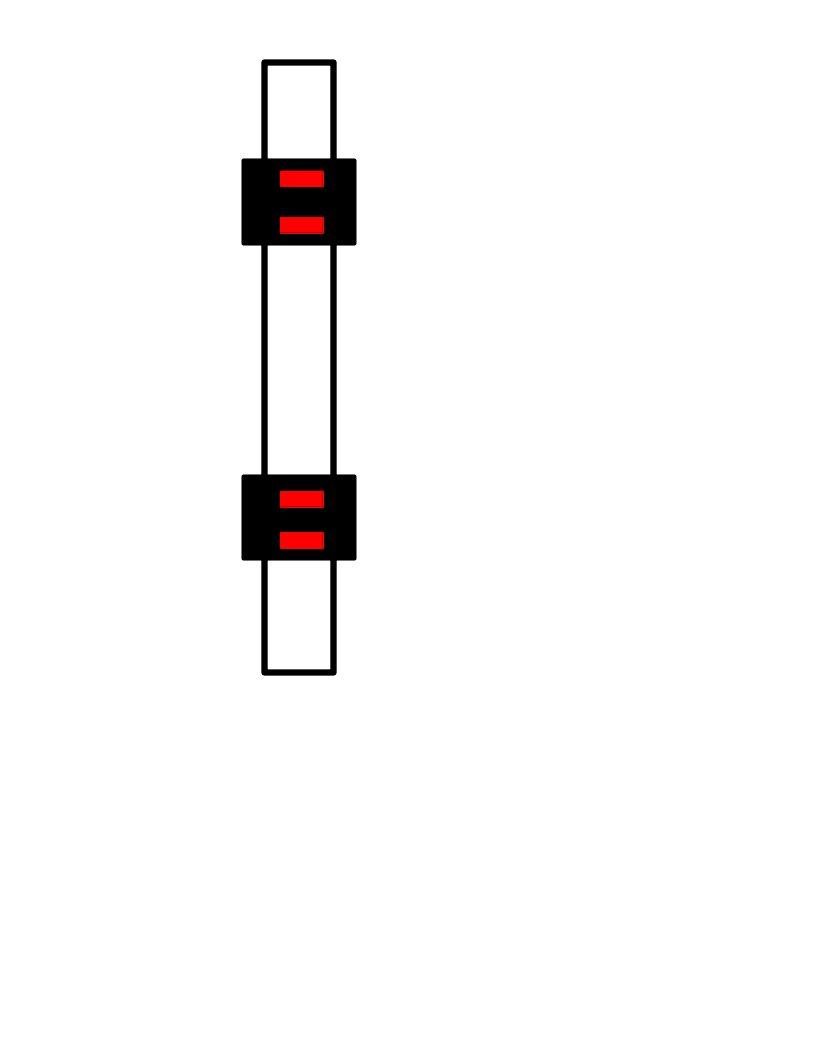
\includegraphics[width=0.23\textwidth,scale=0.2]{reticules.png}
\caption{\label{fig:reticules}Reticules}
\end{wrapfigure}

The placement of the reticule does not limit the level control to this level. Level control is relative to the reticules and may be set to maintain levels at an offset above or below the level of the reticules. In the simplist case, it is convenient to position the reticule assemblies so that the two red bars are placed to surround the desired liquid level.  This would correspond to an offset of zero for the liquid level to be maintained.



\subsubsection*{Vessels}
1) the region of the image where the meniscus will be visible, for each vessel and intensity and contrast settings that have been selected by the user.

\subsection*{Lighting}
Valid levels cannot be obtained if the EvoStat chamber is opened, and therefore exposed to normal room lighting.  While the ability to darken the room can substitute for a closed chamber, we haven't had that luxury since being evicted from the Tod Vision's gardening tool shed in the Genome Sciences Building.

Therefore, whenever the level monitoring program is called by the EvoStat and good level readings are not possible, there is no output produced and the EvoStat control program makes operates as if the readings were unchanged.


\subsection*{Growth Conditions}


\bibliography{alevel}{}
\bibliographystyle{unsrt}
\end{document}













